\section{Marco teórico y trabajos relacionados}
\subsection{Gestión de Tickets de Soporte Técnico}
La gestión de incidencias constituye un reto significativo en instituciones públicas y privadas. Con frecuencia, los procesos de atención a solicitudes se realizan de manera manual, lo que conlleva a problemas de trazabilidad, duplicación de casos y pérdida de información crítica. Este contexto motivó el desarrollo de un Sistema de Gestión de Tickets con soporte web y móvil, cuyo propósito es centralizar la información, generar métricas confiables y ofrecer herramientas de comunicación efectivas entre técnicos, usuarios y administradores.

Un sistema de gestión de tickets de soporte combina herramientas simples para registrar solicitudes, categorizarlas, asignarlas a técnicos especializados y hacer seguimiento de su resolución, con algoritmos que optimizan la distribución de carga de trabajo. En la práctica, soluciones similares usan algoritmos de optimización para resolver estos problemas, demostrando que es posible hacer esto de forma eficiente en entornos organizacionales. Comparado con métodos manuales tradicionales, que dependen de la intuición humana y son propensos a errores, el Sistema de Tickets ofrece una alternativa automatizada que ahorra tiempo y reduce frustraciones.

\begin{figure}[h]
\centering
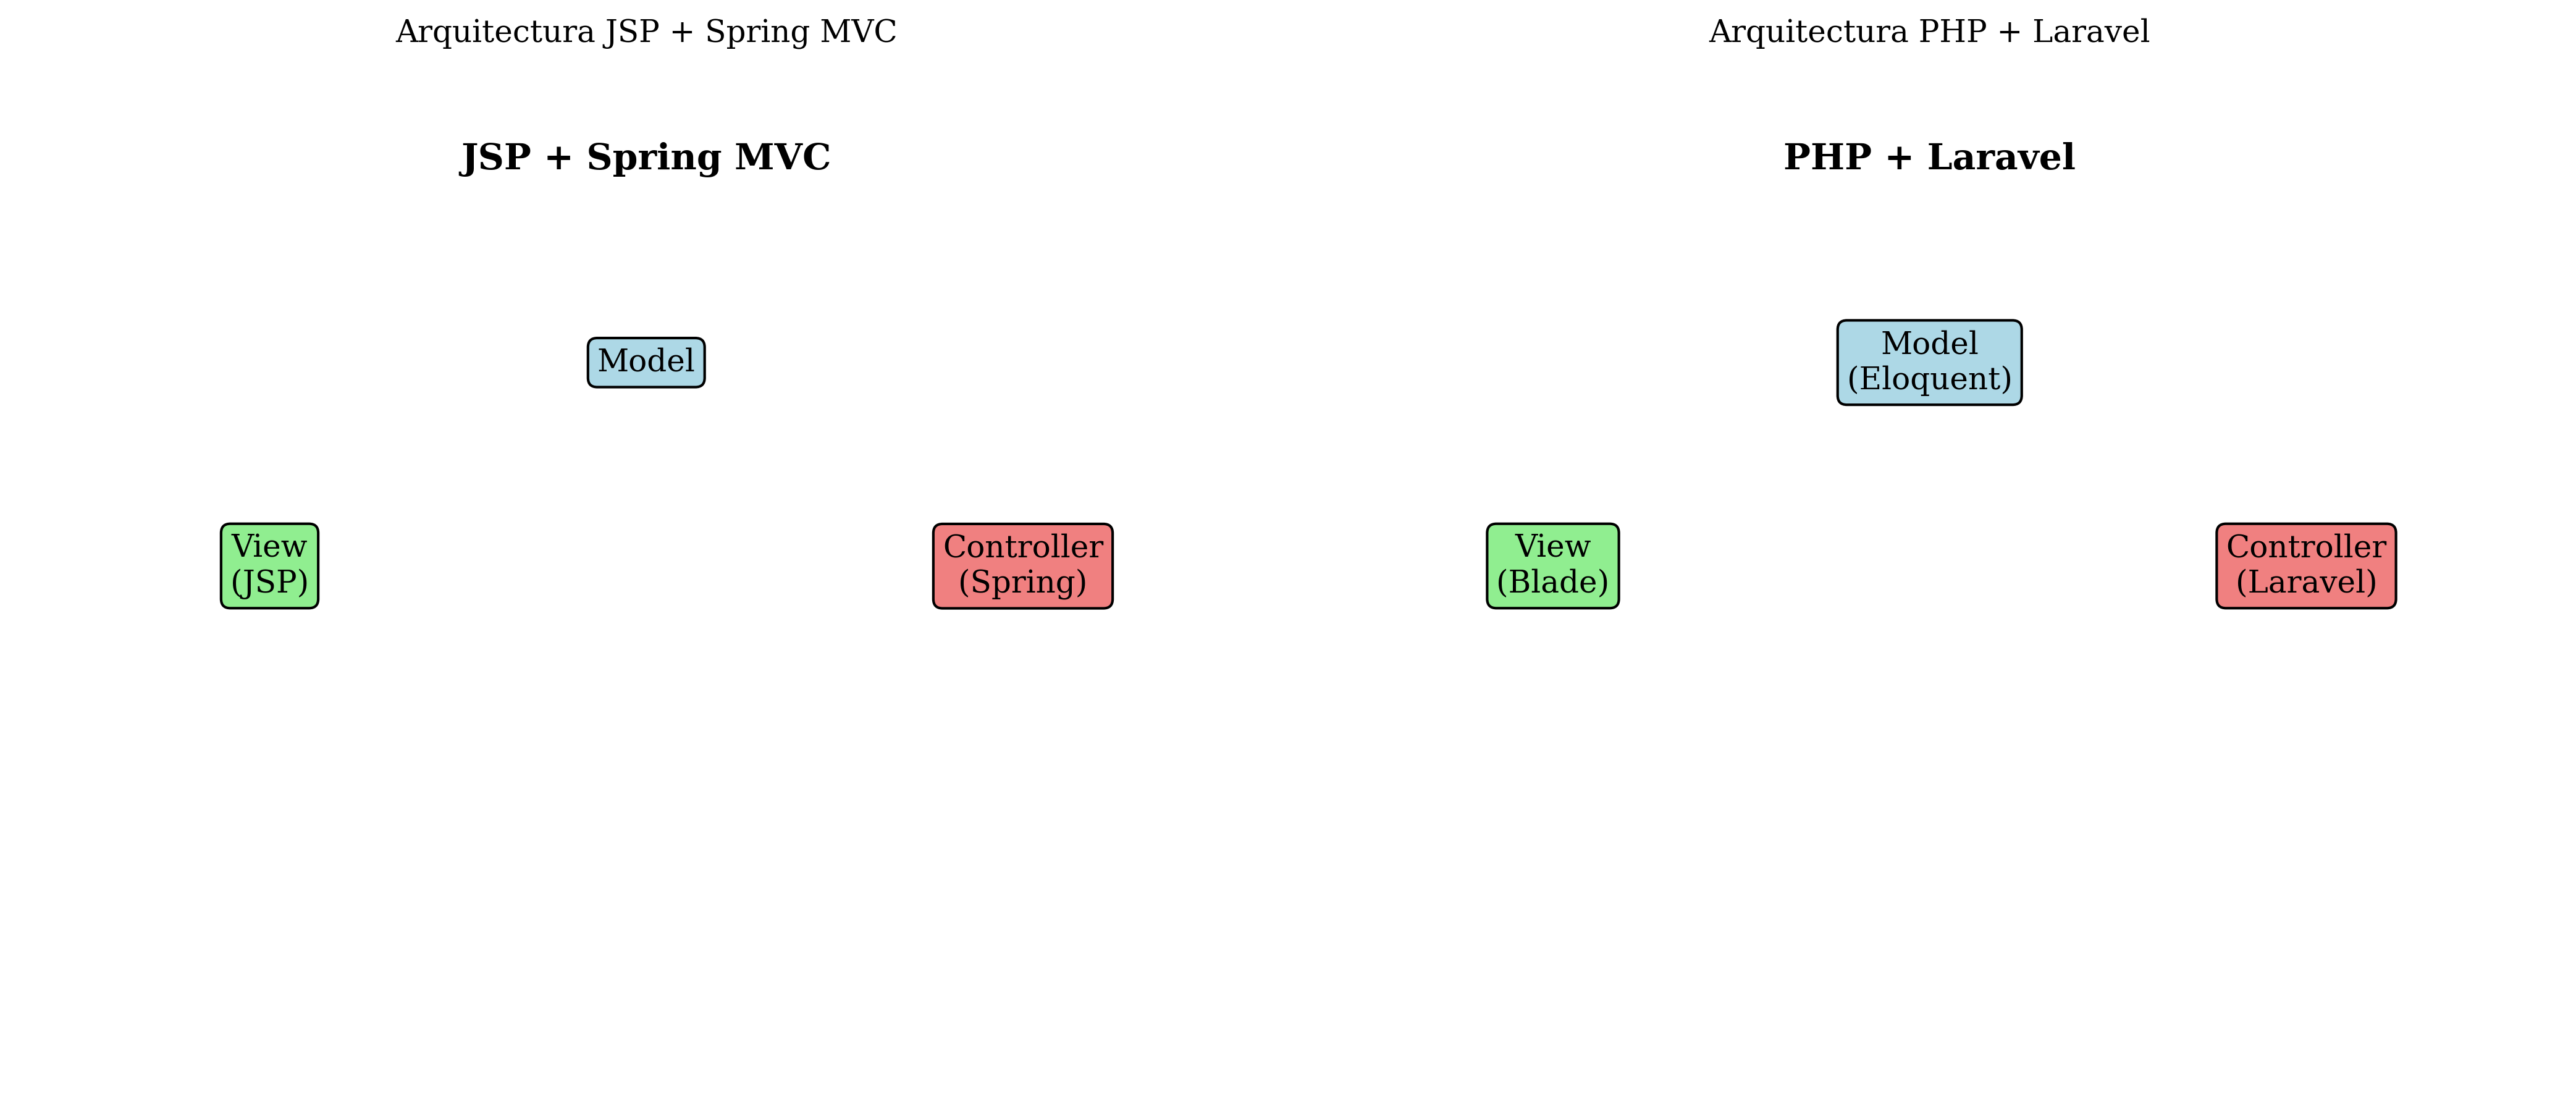
\includegraphics[width=0.8\columnwidth]{graphics/mvc-architecture-jsp-php.png.jpg}
\caption{Arquitectura MVC comparada entre JSP y PHP para aplicaciones cliente-servidor.}
\label{fig:mvc_architecture}
\end{figure}

\subsection{Metodologías Ágiles: Scrum}
La metodología aplicada se fundamentó en el marco ágil Scrum, reconocido por su flexibilidad y orientación a la entrega continua (Alarcón et al., 2021). El trabajo se organizó en sprints de dos semanas, donde cada iteración culminaba con un incremento funcional del sistema. Se llevaron a cabo reuniones de planificación, daily scrums y revisiones de sprint, garantizando retroalimentación constante.

En términos metodológicos, se adoptó Scrum como marco de trabajo (Alarcón et al., 2021), el cual facilita entregas incrementales y fomenta la adaptabilidad del proyecto. La literatura destaca que las metodologías ágiles, aplicadas en conjunto con frameworks modernos, permiten reducir la deuda técnica y obtener productos más cercanos a las necesidades reales de los usuarios (Fernández-Medina et al., 2022).

Desde la perspectiva metodológica, la adopción de Scrum resultó fundamental para gestionar cambios en los requerimientos y mantener un ritmo de entrega constante. Tal como lo plantean Alarcón et al. (2021), la efectividad de Scrum depende de combinarlo con buenas prácticas de documentación y pruebas.

\begin{figure}[h]
\centering
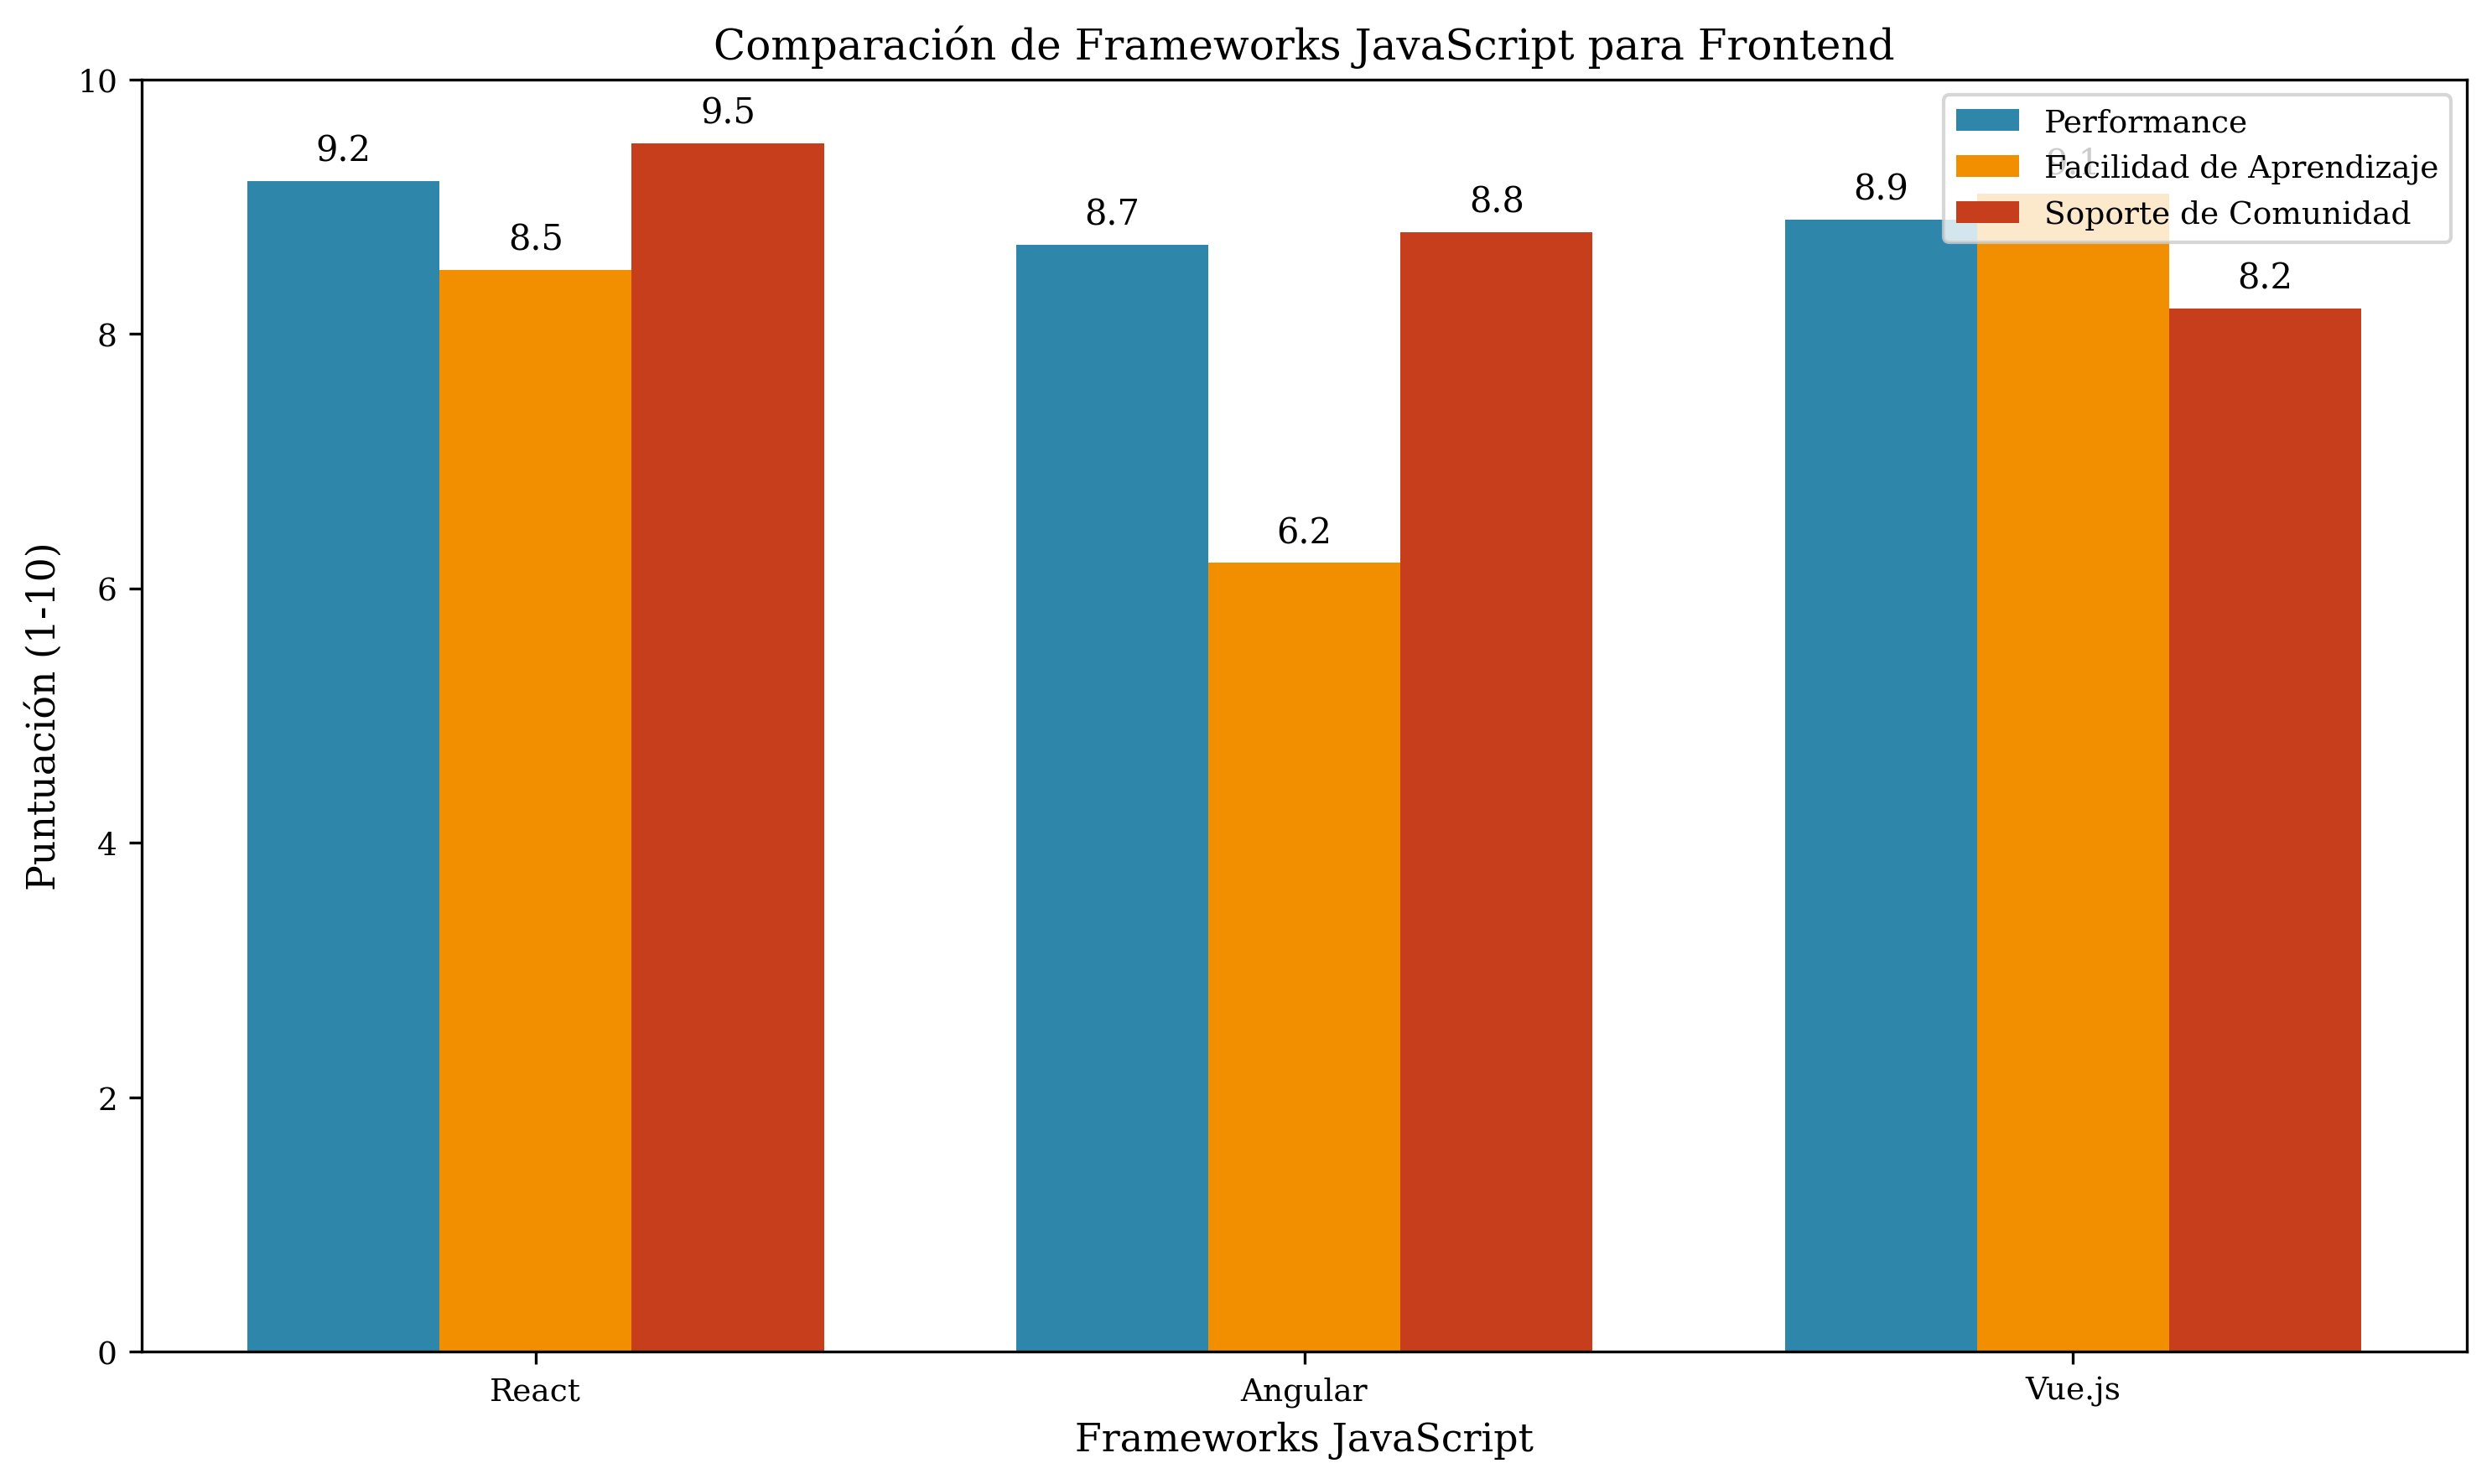
\includegraphics[width=0.8\columnwidth]{graphics/frameworks-javascript.png.jpg}
\caption{Frameworks de JavaScript para desarrollo frontend moderno.}
\label{fig:javascript_frameworks}
\end{figure}

\subsection{Metodologías Ágiles: Scrum en el Sistema de Tickets}
Scrum es como un juego de equipo donde divides el trabajo en rondas cortas llamadas sprints, cada una de unas semanas, para construir el software poco a poco. En el Sistema de Tickets, adoptamos Scrum porque permite responder rápidamente a cambios, como cuando un técnico necesita una nueva funcionalidad para categorizar tickets.

En Scrum, los requerimientos se especifican con historias de usuario, que son simples y enfocadas en el valor para el usuario \cite{izaurralde2013}. A diferencia de métodos tradicionales que requieren planear todo al detalle antes de empezar, Scrum permite empezar con lo básico y refinar en cada sprint mediante reuniones diarias y retrospectivas. Esto hace que el desarrollo sea más adaptable y menos estresante.

Comparado con enfoques waterfall (donde todo se planea de una vez), Scrum en el Sistema de Tickets es como construir una casa habitación por habitación en lugar de diseñar todo el plano primero: puedes ajustar si encuentras un problema, y el resultado final se siente más vivo y útil.

\subsection{Tecnologías Backend: Laravel Framework}
Desde el punto de vista técnico, el backend se desarrolló en Laravel, seleccionado por su arquitectura MVC y sus herramientas nativas como Eloquent ORM, Blade y middleware de seguridad \cite{subecz2021}. La elección se sustentó también en estudios comparativos que muestran la accesibilidad de Laravel frente a Symfony en equipos pequeños \cite{mvc2021}.

Este artículo presenta una introducción completa al framework Laravel, un popular framework PHP para desarrollo web que utiliza la arquitectura MVC (Model-View-Controller) y está basado en el sistema Symfony. Laravel emplea un sistema modular de paquetes que permite expandir aplicaciones con nuevos módulos y reutiliza componentes existentes de otros frameworks para crear aplicaciones seguras y operativas rápidamente. Sus principales características incluyen soporte para diferentes bases de datos, utilidades para desarrollo web, motor de enrutamiento simple y rápido, mayor escalabilidad de aplicaciones web y ahorro considerable de tiempo en el diseño.

Laravel incluye funcionalidades esenciales como el sistema de enrutamiento que maneja las solicitudes HTTP, la arquitectura MVC donde los controladores manejan las peticiones de usuario y la lógica de negocio, los modelos representan los datos y las vistas generan la salida. También cubre aspectos como plantillas Blade para separar la lógica de presentación de la lógica de negocio, sistema de migraciones para manipular estructuras de base de datos, Eloquent ORM para consultas eficientes sin SQL crudo, sistema de autenticación y autorización, middleware para filtrar peticiones HTTP, validación de formularios y modelos, y medidas de seguridad contra ataques comunes.

\begin{figure}[h]
\centering
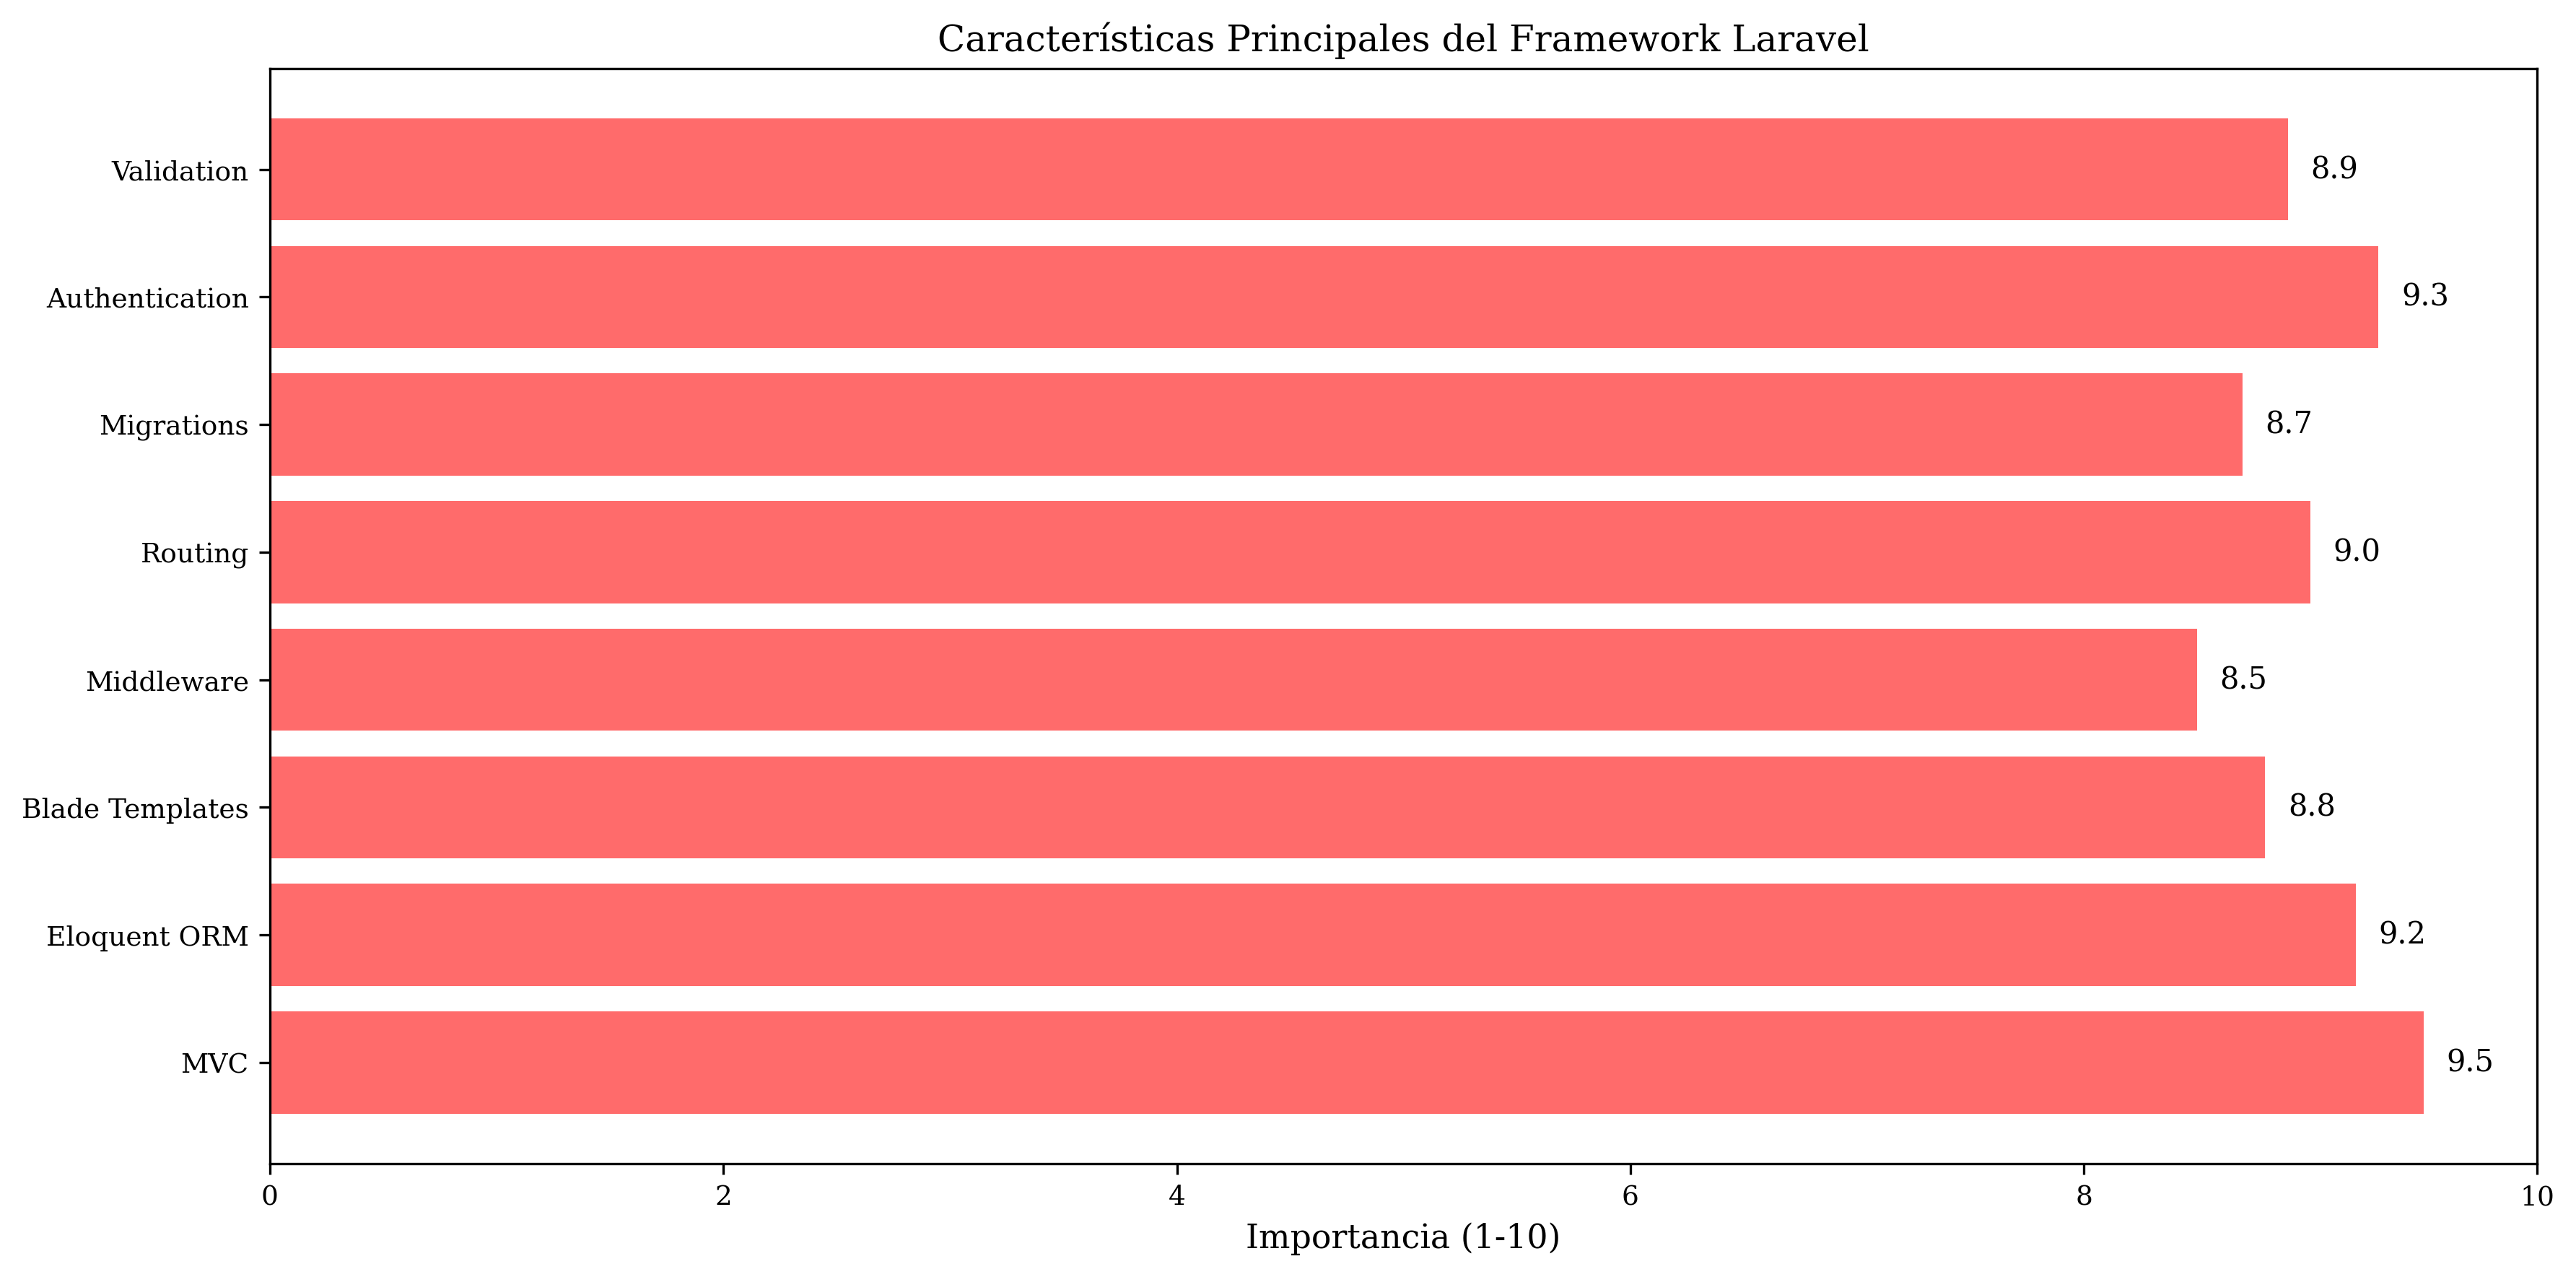
\includegraphics[width=0.8\columnwidth]{graphics/subecz-2021-laravel.png.jpg}
\caption{Framework Laravel para desarrollo web con arquitectura MVC.}
\label{fig:laravel_framework}
\end{figure}

\subsection{Bases de Datos: MySQL en el Sistema de Tickets}
Las bases de datos son como el archivador digital donde guardas toda la información. MySQL es una opción popular porque es gratuita, rápida y fácil de usar, ideal para proyectos como el Sistema de Tickets que necesitan almacenar relaciones complejas, como qué técnico atiende qué ticket en qué categoría \cite{lozano2018}.

MySQL surgió en los 90 como una evolución de sistemas más antiguos, y hoy es una herramienta clave para datos estructurados. Comparado con bases de datos no relacionales como MongoDB, que son más flexibles para datos irregulares pero pueden ser menos consistentes, MySQL garantiza que todo esté bien organizado con el modelo ACID \cite{saltos2022}. En el Sistema de Tickets, optamos por MySQL porque nuestros datos (tickets, técnicos, categorías, usuarios) tienen relaciones claras que necesitan integridad, y lo ejecutamos en XAMPP para desarrollo local, con phpMyAdmin para gestionar todo sin complicaciones.

\begin{figure}[h]
\centering
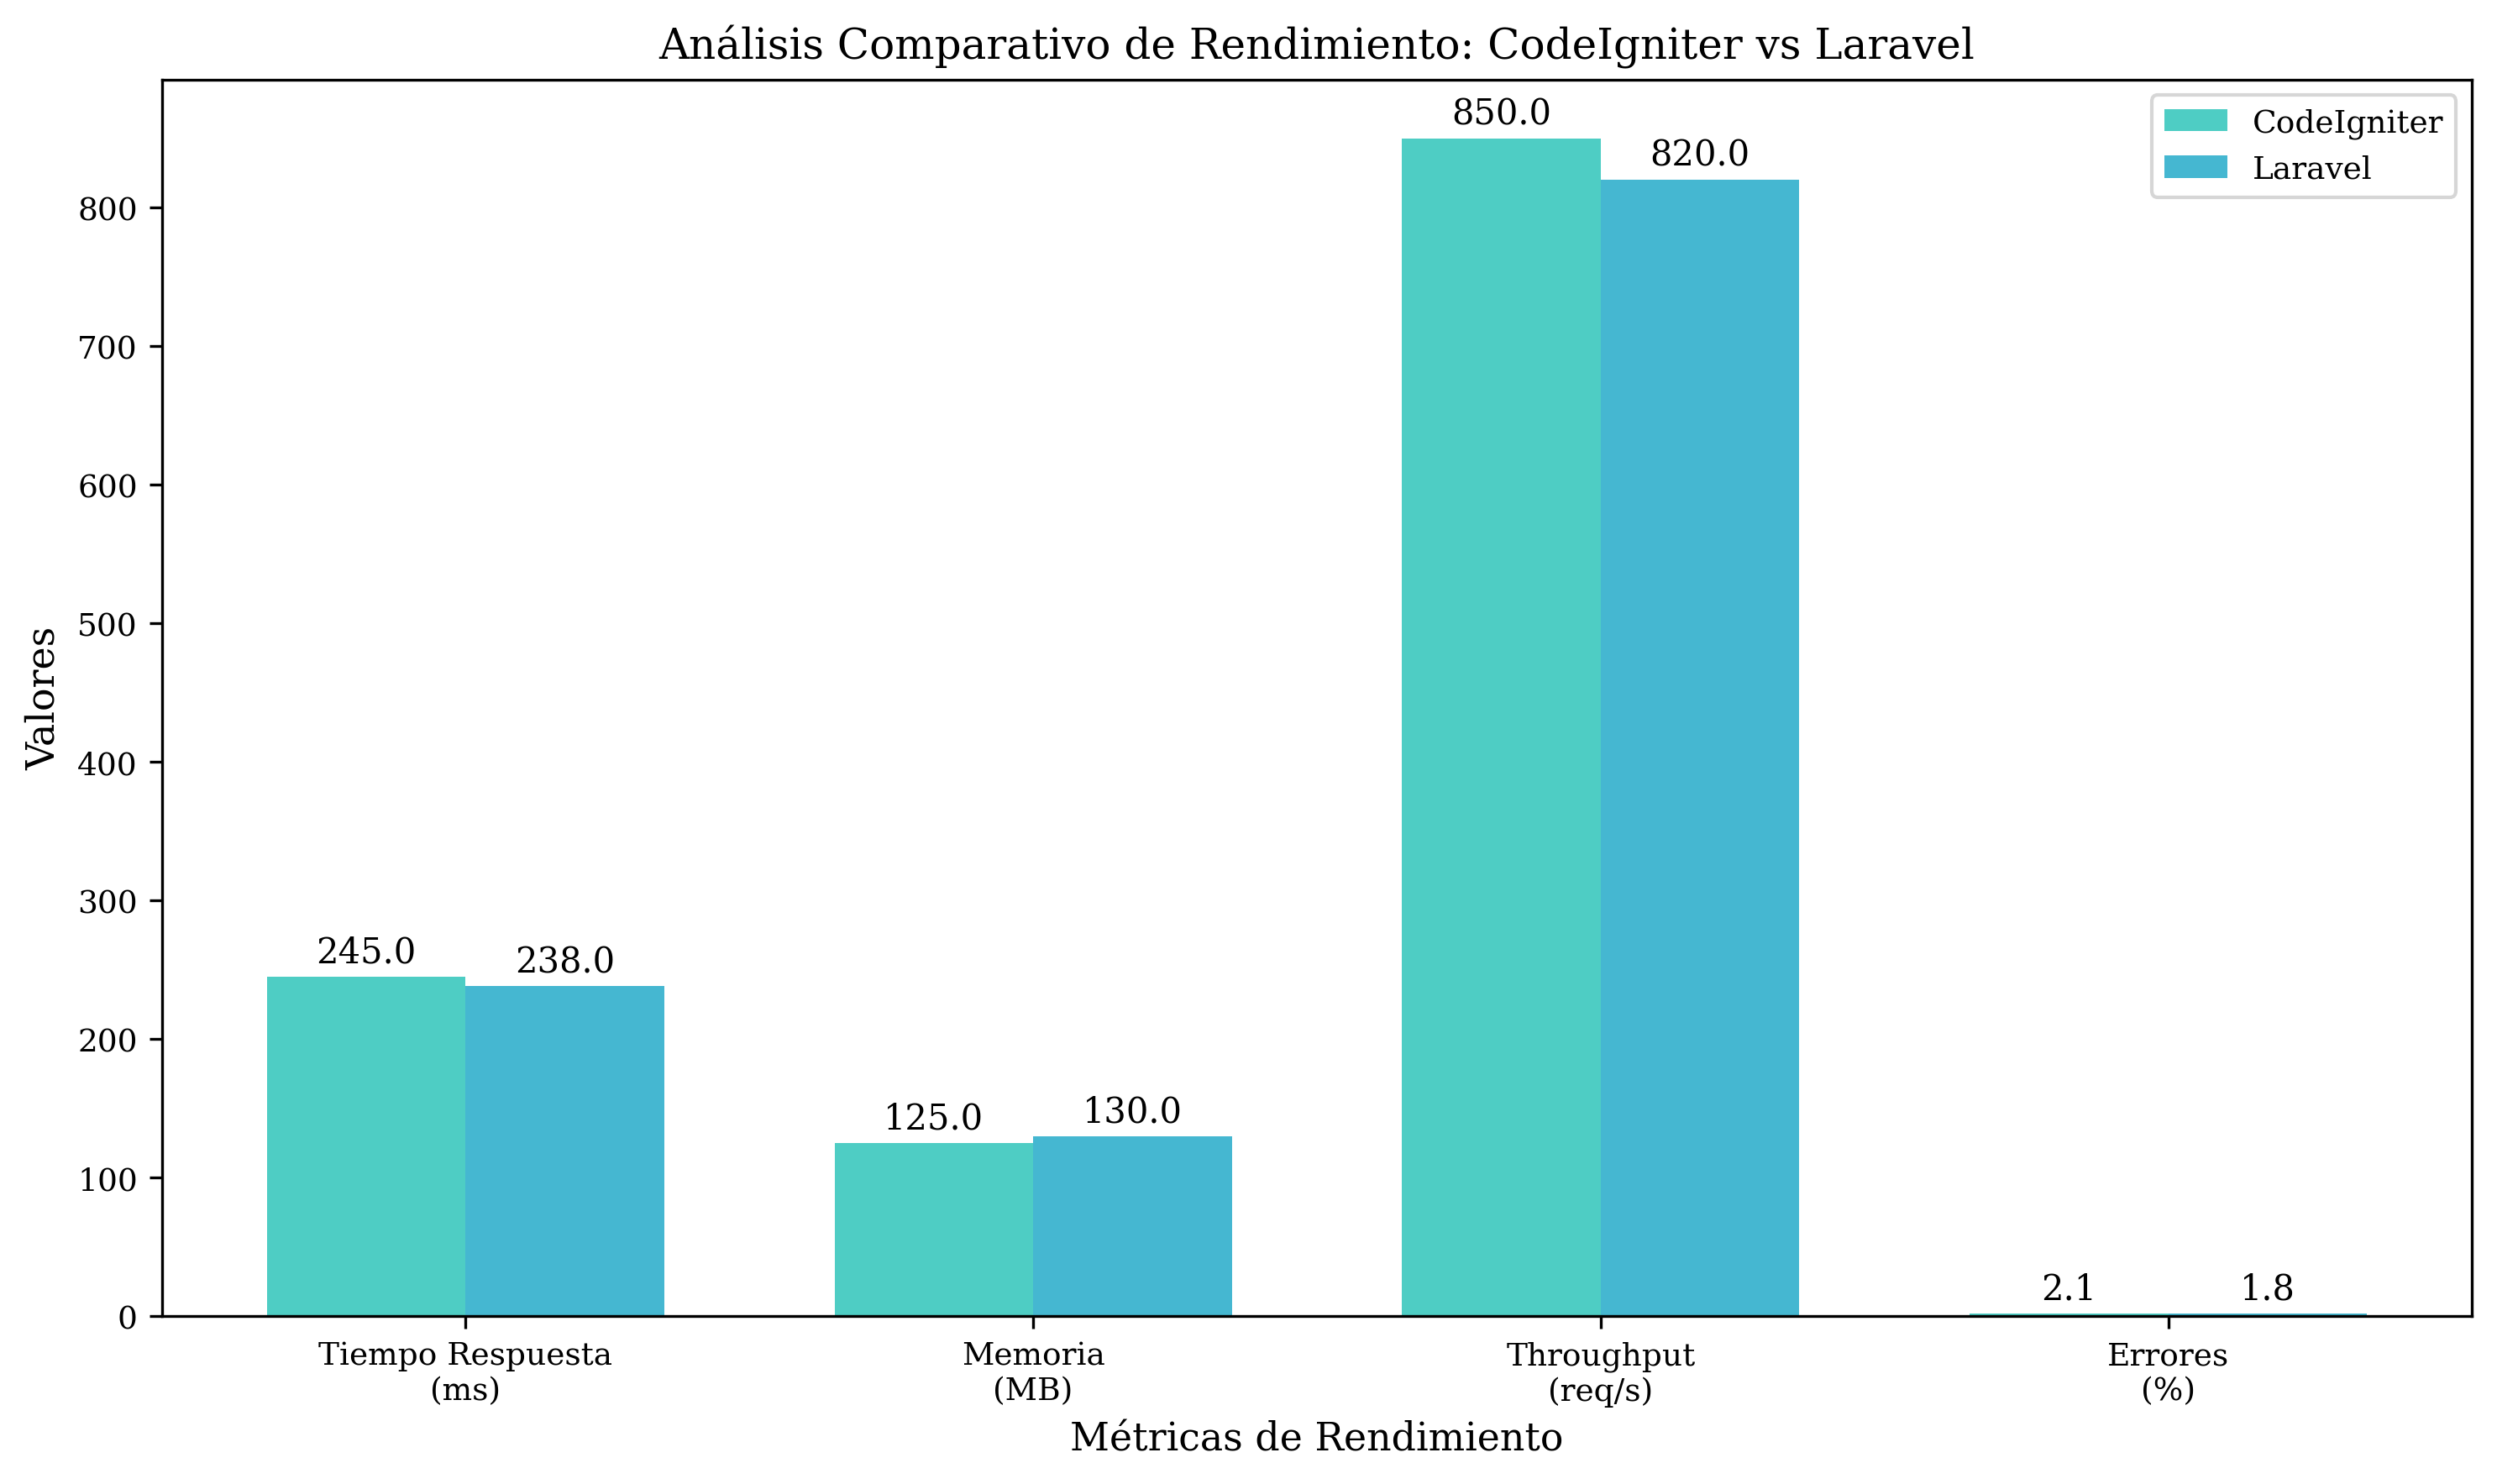
\includegraphics[width=0.8\columnwidth]{graphics/codeigniter-laravel-performance.png.jpg}
\caption{Análisis comparativo de rendimiento entre CodeIgniter y Laravel.}
\label{fig:codeigniter_laravel}
\end{figure}

\begin{figure}[h]
\centering

\includegraphics[width=0.8\columnwidth]{graphics/accesibilidad-web.png}
\caption{Guías para el desarrollo web accesible siguiendo estándares W3C.}
\label{fig:accesibilidad_web}
\end{figure}

\subsection{Interfaces Web y Móviles: React y React Native}
En el frontend, React fue adoptado gracias a su enfoque en componentes reutilizables y su curva de aprendizaje intermedia (Kaur & Kaur, 2020). La aplicación móvil, inicialmente desarrollada para Android, integra funcionalidades clave como notificaciones push y carga de evidencias multimedia. Estudios previos demuestran que React Native es una solución idónea para expandir la compatibilidad a iOS sin necesidad de reescribir la lógica principal (Silva et al., 2022).

Los frameworks de JavaScript, como React, Angular y Vue, han revolucionado la forma en que se desarrollan aplicaciones modernas, proporcionando herramientas y metodologías que facilitan la creación de interfaces dinámicas e interactivas. Entre las principales características de estos frameworks se encuentran la modularidad, la reutilización de componentes y la optimización del rendimiento. React se basa en componentes reutilizables que facilitan la construcción de interfaces, mientras que React Native permite expandir la compatibilidad a iOS sin necesidad de reescribir la lógica principal.

En cuanto al frontend, React se consolidó como la mejor opción para construir una interfaz moderna y eficiente, respaldado por investigaciones que lo destacan frente a Angular y Vue en términos de flexibilidad (Kaur & Kaur, 2020; Singh & Kaur, 2020). La posibilidad de evolucionar hacia React Native fortalece la proyección multiplataforma, coincidiendo con Silva et al. (2022).

\subsection{Arquitectura Modular y Microservicios}
La arquitectura del Sistema de Tickets es modular, como construir con bloques Lego: cada parte (backend, frontend, móvil) es independiente, pero encaja perfectamente. Esto facilita mantener y expandir el sistema, como agregar nuevas funciones sin romper lo existente.

Comparado con arquitecturas monolíticas (todo en un bloque grande), la modularidad en el Sistema de Tickets permite actualizaciones más seguras y escalabilidad. La coexistencia de requerimientos tradicionales con historias de usuario asegura que tengamos lo mejor de ambos mundos: precisión y flexibilidad \cite{izaurralde2013}.

\subsection{APIs RESTful y Autenticación JWT}
Para garantizar calidad y seguridad, se implementaron procesos de pruebas automatizadas en componentes críticos, siguiendo buenas prácticas de integración continua y despliegue seguro \cite{seguridad2020}. Las APIs son como puentes que conectan las partes del Sistema de Tickets. Usamos RESTful para intercambiar datos de forma segura y eficiente, con JWT para autenticar usuarios sin guardar sesiones en el servidor.

Comparado con APIs más antiguas, REST es simple y escalable, ideal para apps móviles. En el Sistema de Tickets, documentamos todo con Swagger para que sea fácil probar y entender, mejorando la colaboración entre equipos.

\begin{figure}[h]
\centering
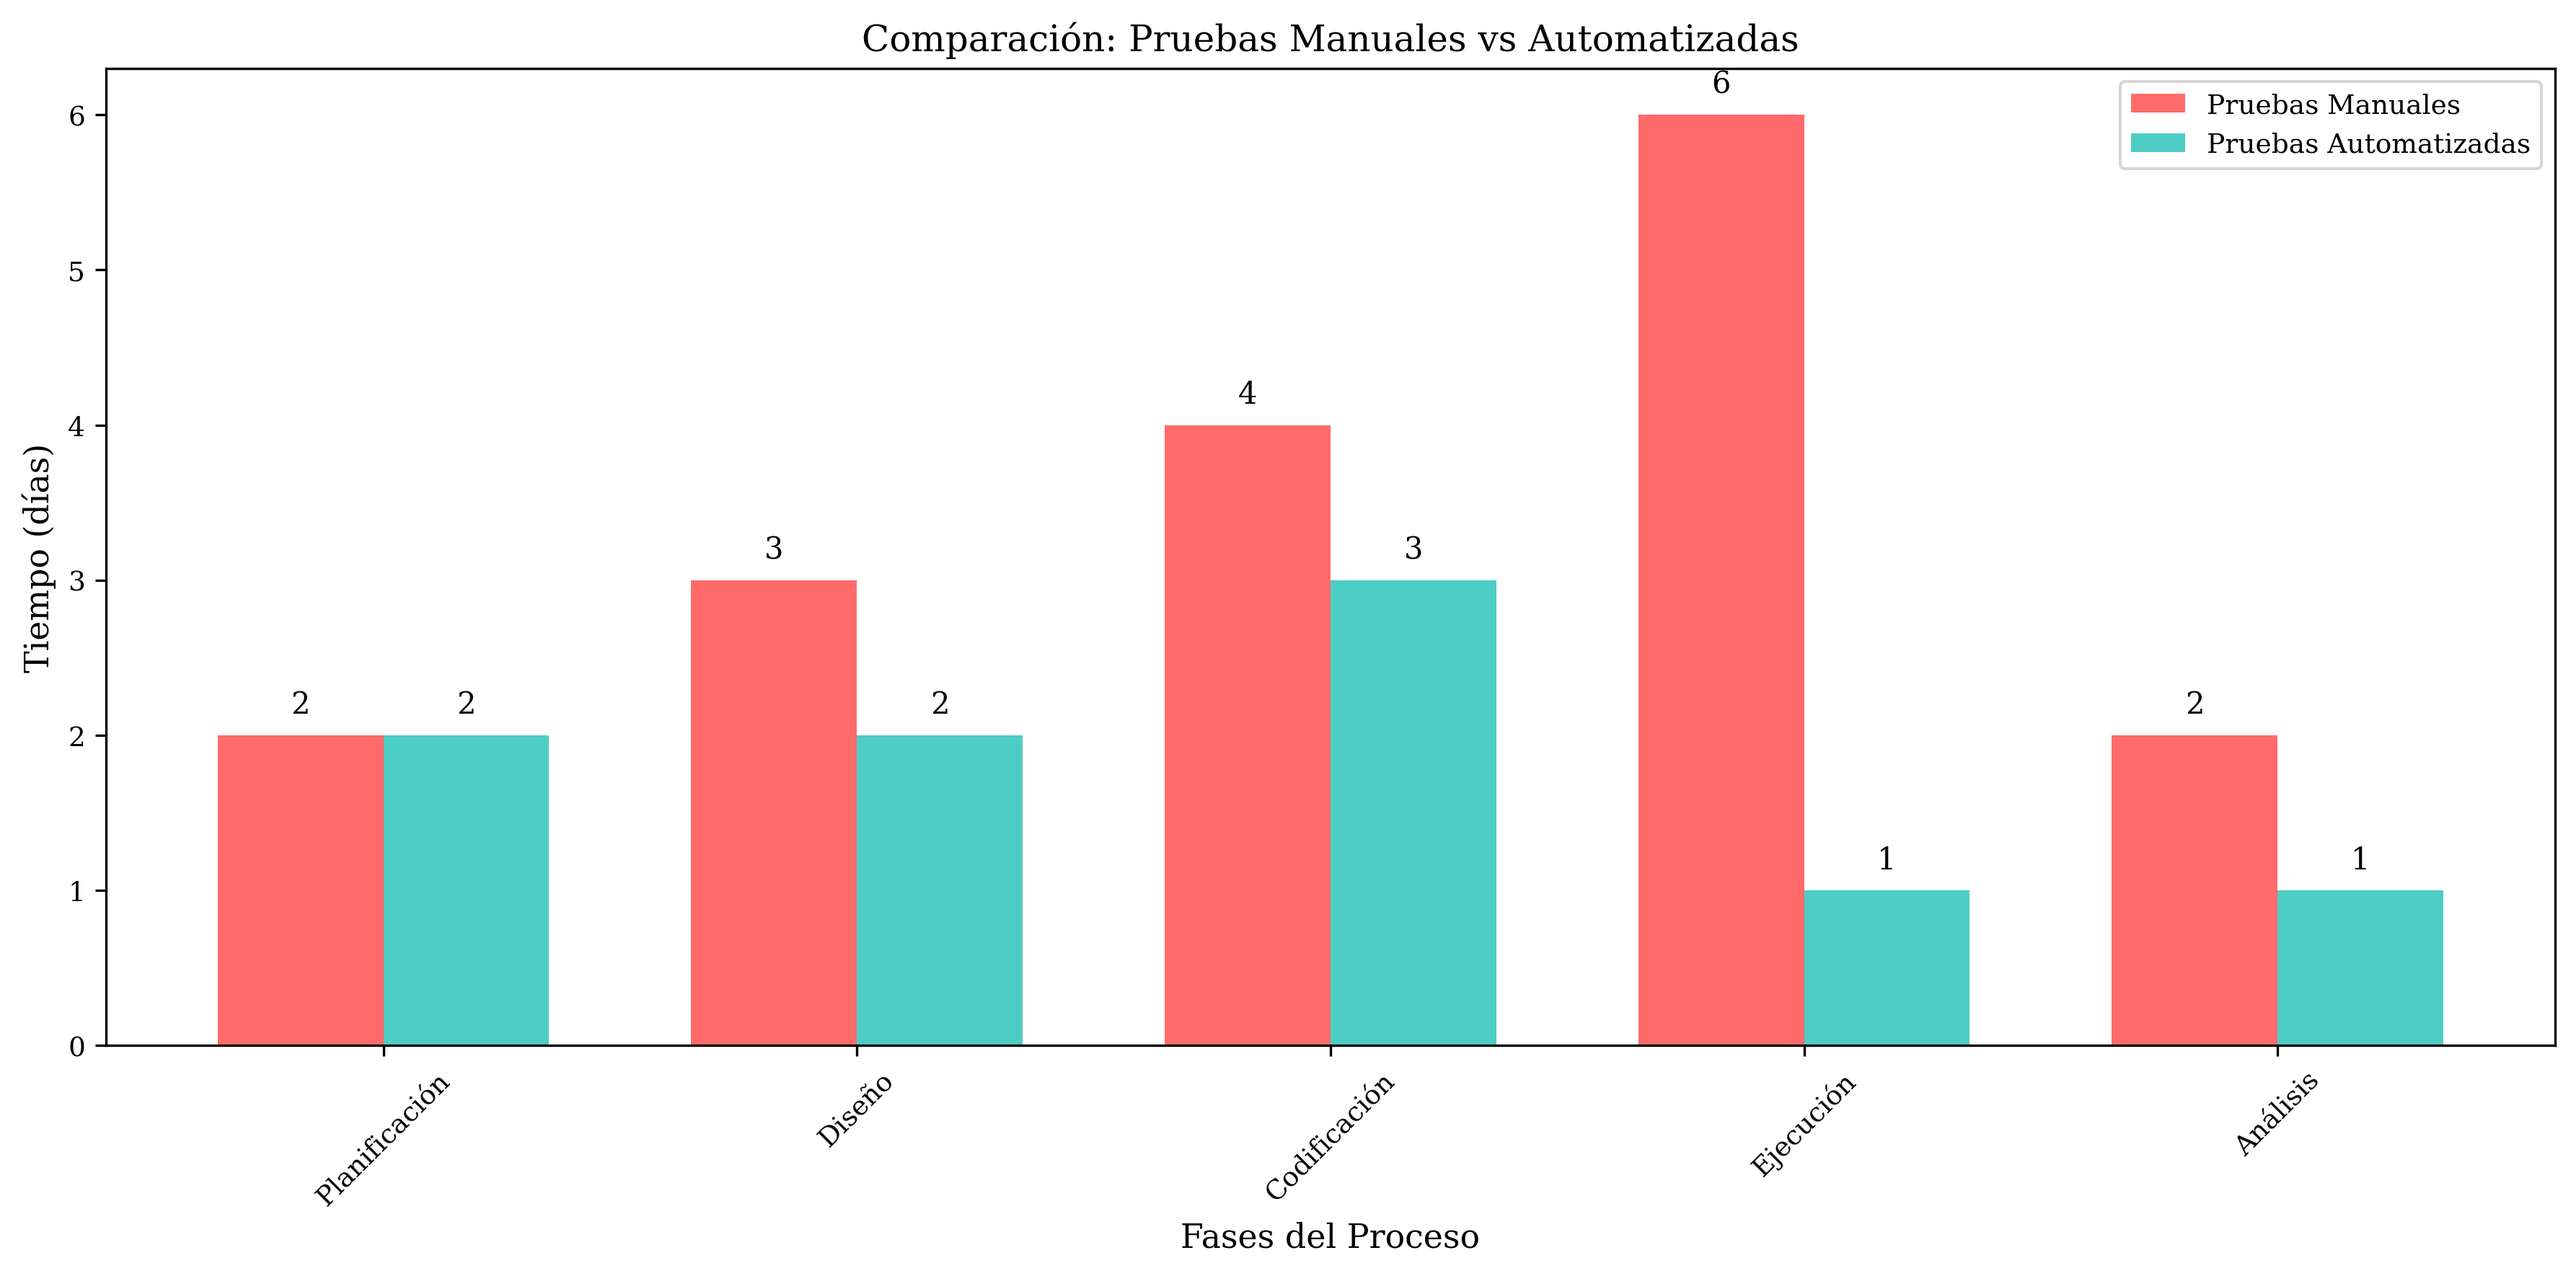
\includegraphics[width=0.8\columnwidth]{graphics/automatizacion-pruebas.png.jpg}
\caption{Proceso de automatización de pruebas para aplicaciones web.}
\label{fig:automatizacion_pruebas}
\end{figure}

\subsection{Docker: Contenerización para Despliegue}
Para garantizar calidad y seguridad, se implementaron procesos de pruebas automatizadas en componentes críticos, siguiendo buenas prácticas de integración continua y despliegue seguro \cite{seguridad2020}. Docker es como empaquetar el Sistema de Tickets en una caja portable que funciona igual en cualquier máquina. Resuelve problemas de compatibilidad, reduciendo tiempos de despliegue de días a horas.

Comparado con máquinas virtuales, que simulan computadoras completas, Docker es más ligero y eficiente, perfecto para orquestar servicios en el Sistema de Tickets sin complicaciones.

\begin{figure}[h]
\centering
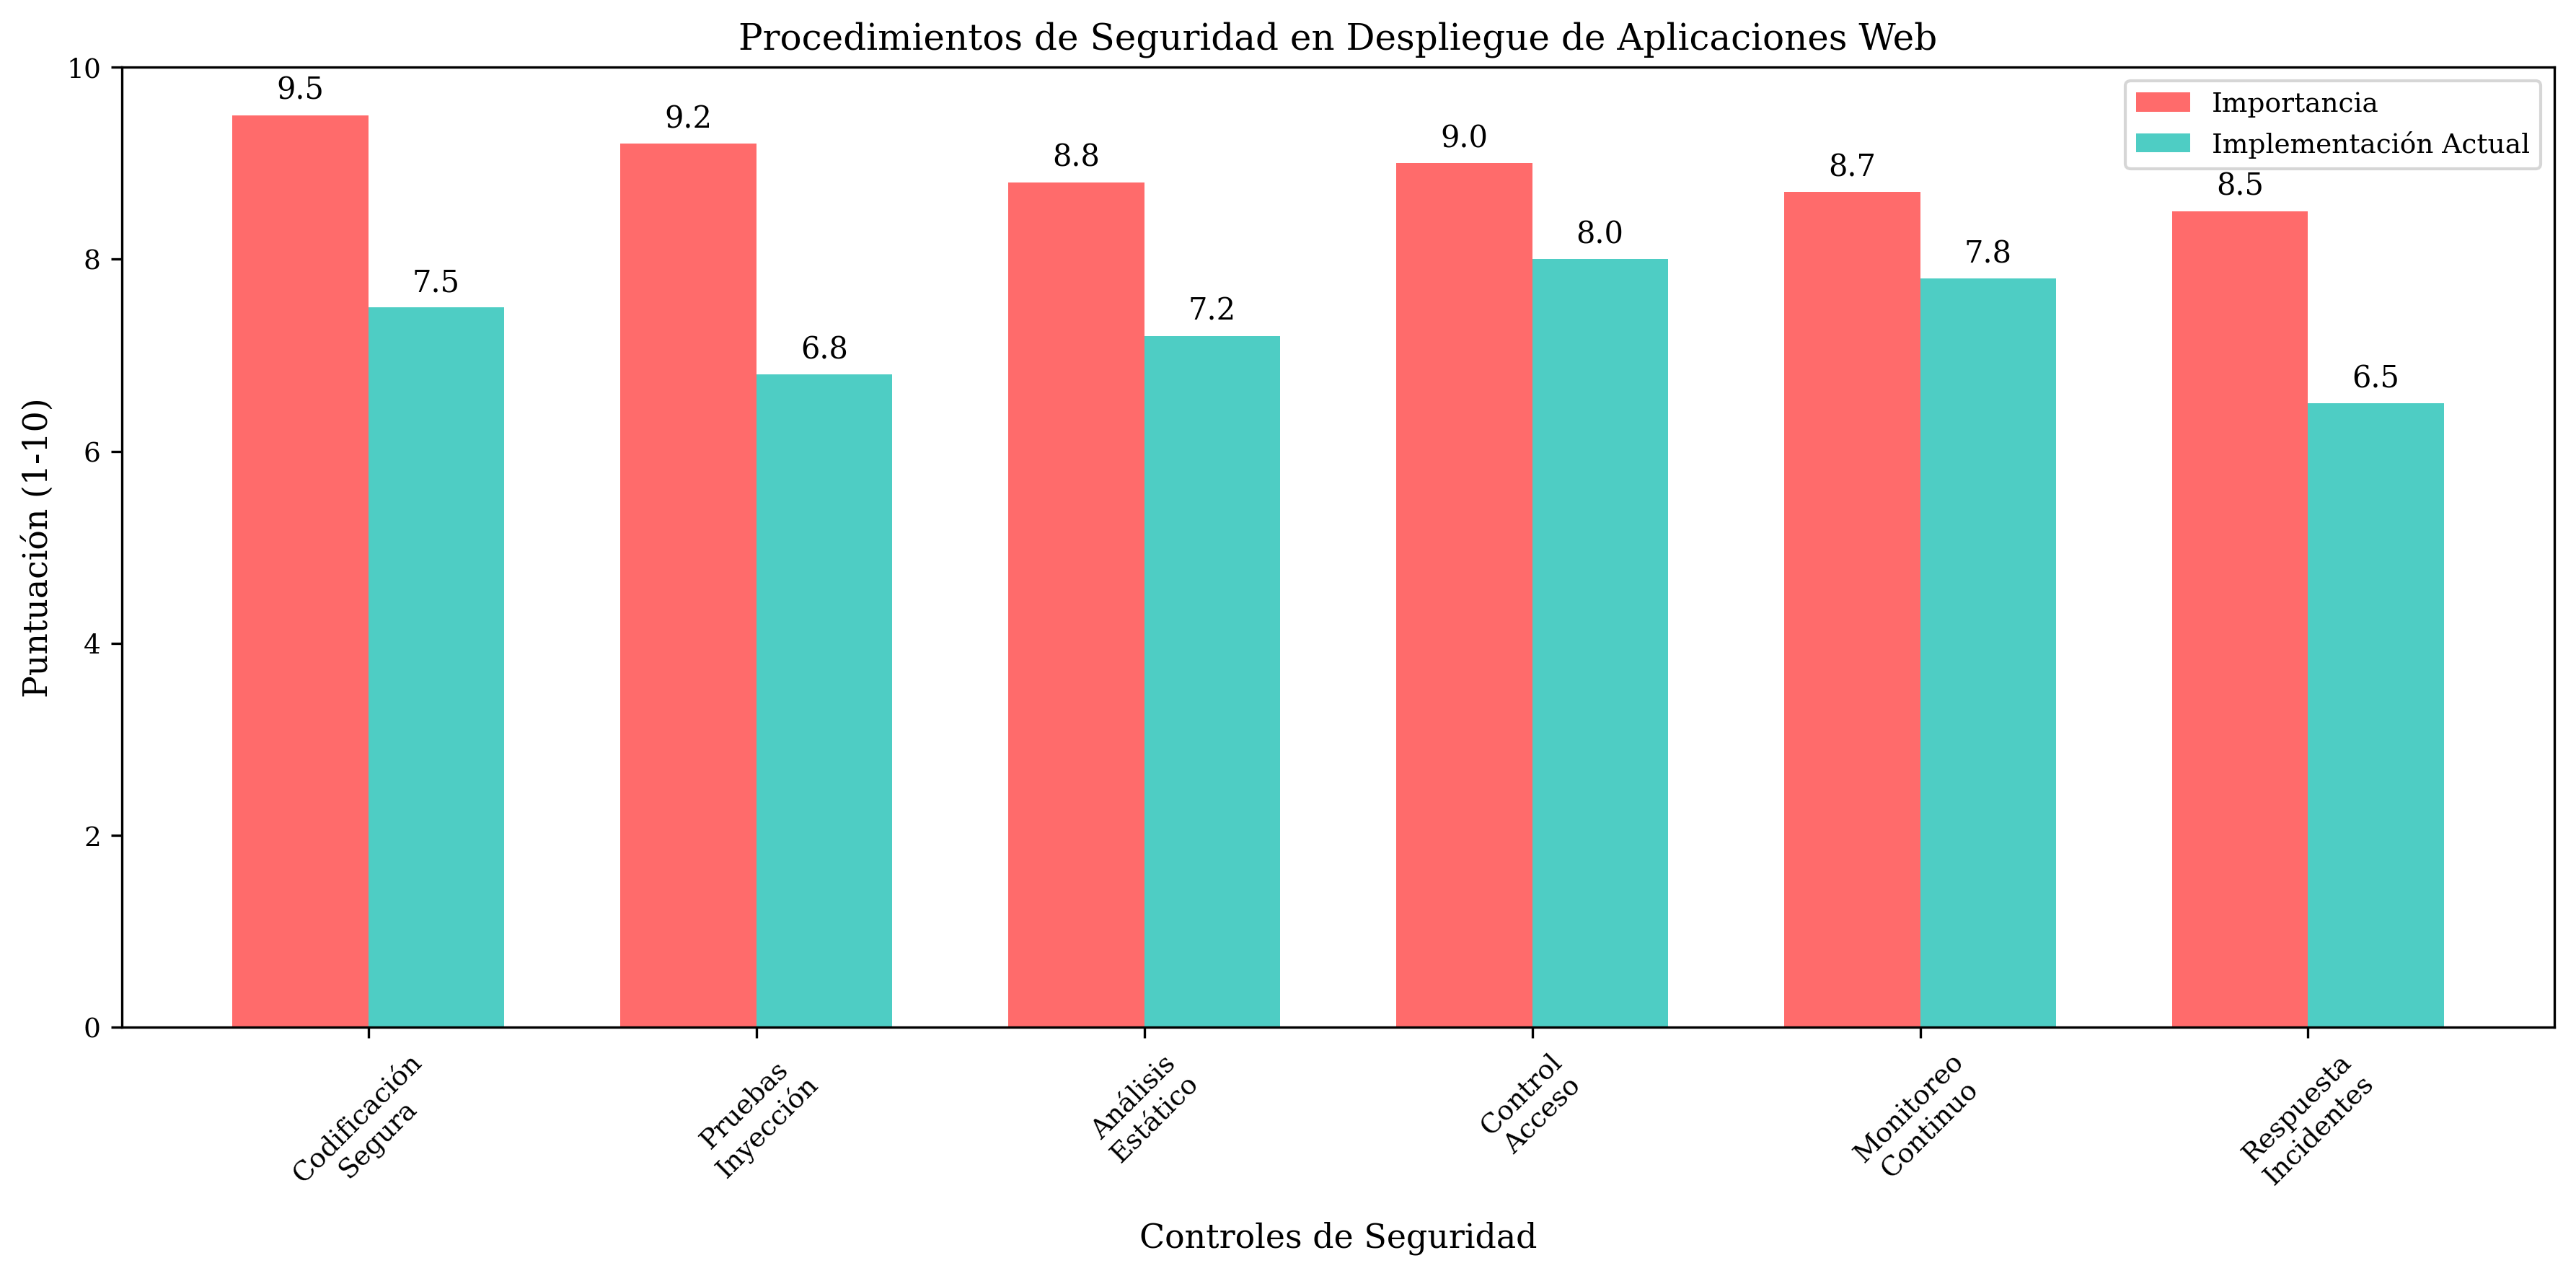
\includegraphics[width=0.8\columnwidth]{graphics/seguridad-despliegue.png.jpg}
\caption{Procedimiento para la seguridad del proceso de despliegue de aplicaciones web.}
\label{fig:seguridad_despliegue}
\end{figure}